\documentclass[11pt,a4paper,twoside]{article}

% Input encoding and basic packages
\usepackage[utf8]{inputenc}
\usepackage{amsmath, amssymb}
\usepackage{graphicx}
\usepackage{tcolorbox}
\usepackage{xcolor}
\usepackage{geometry}
\usepackage{wrapfig}
\usepackage{titlesec}
\usepackage{fancyhdr}
\usepackage{caption}
\usepackage{float}
\usepackage{hyperref}
\usepackage{subcaption}
\usepackage{fontspec}

% Fonts for paragraphs and titles
\usepackage{sectsty} % Allows custom section styles
\usepackage{helvet}  % Default sans-serif font
\usepackage{times}   % Example serif font for body text
% Define custom fonts
\setmainfont{Poppins} % Main font for body text
\newfontfamily\titlesfont{Anonymous Pro} % Font for titles

\raggedbottom

% Define custom colors
\definecolor{cherenkovblue}{RGB}{55, 139, 230}

% Adjust default font sizes (Explicitly set sizes)
\renewcommand{\normalsize}{\fontsize{9}{11}\selectfont} % Smaller body text: 9pt font with 11pt line spacing
\renewcommand{\small}{\fontsize{8}{10}\selectfont}
\renewcommand{\footnotesize}{\fontsize{7}{9}\selectfont}

% Force a new page before every \section and make titles all caps
\makeatletter
\let\oldsection\section
\renewcommand{\section}{\clearpage\@startsection {section}{1}{\z@}%
  {-3.5ex \@plus -1ex \@minus -.2ex}%
  {2.3ex \@plus.2ex}%
  {\titlesfont\fontsize{14}{16}\bfseries\color{cherenkovblue}\MakeUppercase}}
\makeatother

% Custom subsection font
\subsectionfont{\titlesfont\fontsize{12}{14}\bfseries\color{cherenkovblue}} % Subsection: 12pt font, bold, blue

% Customize spacing
\setlength{\parskip}{6pt} % Add spacing between paragraphs
\setlength{\parindent}{0pt} % Remove paragraph indentation
\setlength{\itemsep}{4pt} % Add spacing between list items

% Customize itemize bullets
\renewcommand\labelitemi{--} % Use dashes instead of bullets


% Define fancy header and footer
\fancypagestyle{plain}{
    \fancyhf{} % Clear all header and footer fields
} % Default plain style for title and index pages

\fancypagestyle{post-index}{
    \fancyhf{} % Clear all header and footer fields
    \fancyhead[LE]{\textit{Simone Pagliuca}}
    \fancyhead[RO]{\textit{Genetic Algorithm}}
    \fancyfoot[LE,RO]{\thepage}
    \renewcommand{\headrulewidth}{0.4pt}
    \renewcommand{\footrulewidth}{0.4pt}
}


\begin{document}

\thispagestyle{plain}

% Title with Titles Font (Anonymous Pro)
{\titlesfont\fontsize{18}{28}\textbf{\color{cherenkovblue}{GENETIC ALGORITHM: \\ IMPLEMENTATION AND OPTIMIZATION}}}\\
{\titlesfont\fontsize{10}{12}\color{cherenkovblue} Nuclear Engineering - Politecnico di Milano}\\

\vspace{-10pt}

% Author information with Main Font (Poppins)
{\normalsize\textbf{Pagliuca Simone}} \\
{\footnotesize\textit{simone1.pagliuca@mail.polimi.it}} \\

\vspace{15pt}

% Course and Academic Year
{\footnotesize\textbf{Course:} Advanced Topics for Nuclear Engineering}\\
{\footnotesize\textbf{Academic year:} 2024/2025}

% Horizontal rule
\vspace{10pt}
\centerline{\rule{1.0\textwidth}{0.4pt}}

\vspace{15pt}

% Abstract with Titles Font for Heading, Main Font for Body
\begin{minipage}{1\textwidth}
    \noindent {\titlesfont\fontsize{12}{14}\textbf{\color{cherenkovblue} Abstract:}} 
    {\normalsize
    The objective of this project is to explore the implementation and optimization of a Genetic Algorithm (GA) solver to minimize the Styblinski-Tang function. This report details the approach taken for coding the GA solver, a parametric study on its performance, and the results obtained. The Styblinski-Tang function, with a known global minimum, serves as a benchmark for evaluating the accuracy and efficiency of the algorithm.
    }
\end{minipage}

\vspace{20pt}

% Key-words box with Titles Font
\begin{tcolorbox}[arc=0pt, boxrule=0pt, colback=cherenkovblue!60, width=\textwidth, colupper=white]
    {\titlesfont\fontsize{10}{10}\textbf{Key-words:}} Genetic Algorithm, Optimization, Algorithm Performance
\end{tcolorbox}

\vspace{12pt}

% Nomenclature

\newpage


\pagestyle{post-index}

\section{Code Description}
The Styblinski-Tang function is used as the fitness function for this problem. Since the GA solver is designed to minimize the function, the "fittest individual" is the one with the minimum value. \\

The algorithm consists of the following steps. Except for initialization, each step offers two possible approaches that can be selected individually and will be discussed in detail later.

    \paragraph{Initialization:} The population is initialized by randomly choosing elements within given boundaries.
    \paragraph{Selection:}
    \begin{itemize}
        \item \textit{Tournament Selection:} For each place in the population, a subset of the population of given dimension is randomly chosen, the fittest individual among the subset is chosen.
        \item \textit{Roulette Selection:} For each place in the population,  a subset of the population of given dimension is randomly chosen, probability-weighted selection based on fitness values determines the survoivor.
    \end{itemize}
    \paragraph{Crossover:} 
    \begin{itemize}
        \item \textit{Punnet Crossover:} This is something i made up, for each element of the population there is a given probability that we randomly select two parents, combine their x and y components, evaluate the 4 possible outcomes and selects the best one.
        \item \textit{Bit Crossover:} For each element of the population there is a given probability that we randomly select two parents then swap a randomly chosen portion of bits from the first 20 digits of the floating-point binary representations (this avoids changing the orders of magnitude).
    \end{itemize}
    \paragraph{Mutation:}
    \begin{itemize}
        \item \textit{Redefine Mutation:} For each element of the population there is a given probability to reinitialize its variables.
        \item \textit{Bit Mutation:} For each element of the population there is a given probability to flip a random bit of a gene's binary representation (again, this effects only the mantissa of the floating rapresentation).
    \end{itemize}


\section{Parametric Study}
A parametric study was conducted to evaluate the impact of all parameters on solver performance. The first step focused on assessing accuracy, as the analytical solution is known. Accuracy is defined as follows:
\begin{equation}
    a = 1 - |{Sol_{GA} - Sol_{analytical}}|
\end{equation}


\subsection{Overall View}

Figure \ref{fig:overall} shows that as the population size increases, the algorithm's accuracy improves. Certain combinations stand out as particularly reliable, including TBB (Tournament - Bit Crossover - Bit Mutation), TBR (Tournament - Bit Crossover - Redefine Mutation), and TPR (Tournament - Punnett Crossover - Redefine Mutation).

For the following analysis, only combinations with an accuracy of $a > 0.99$ will be considered.
\begin{figure}[H]
    \centering
    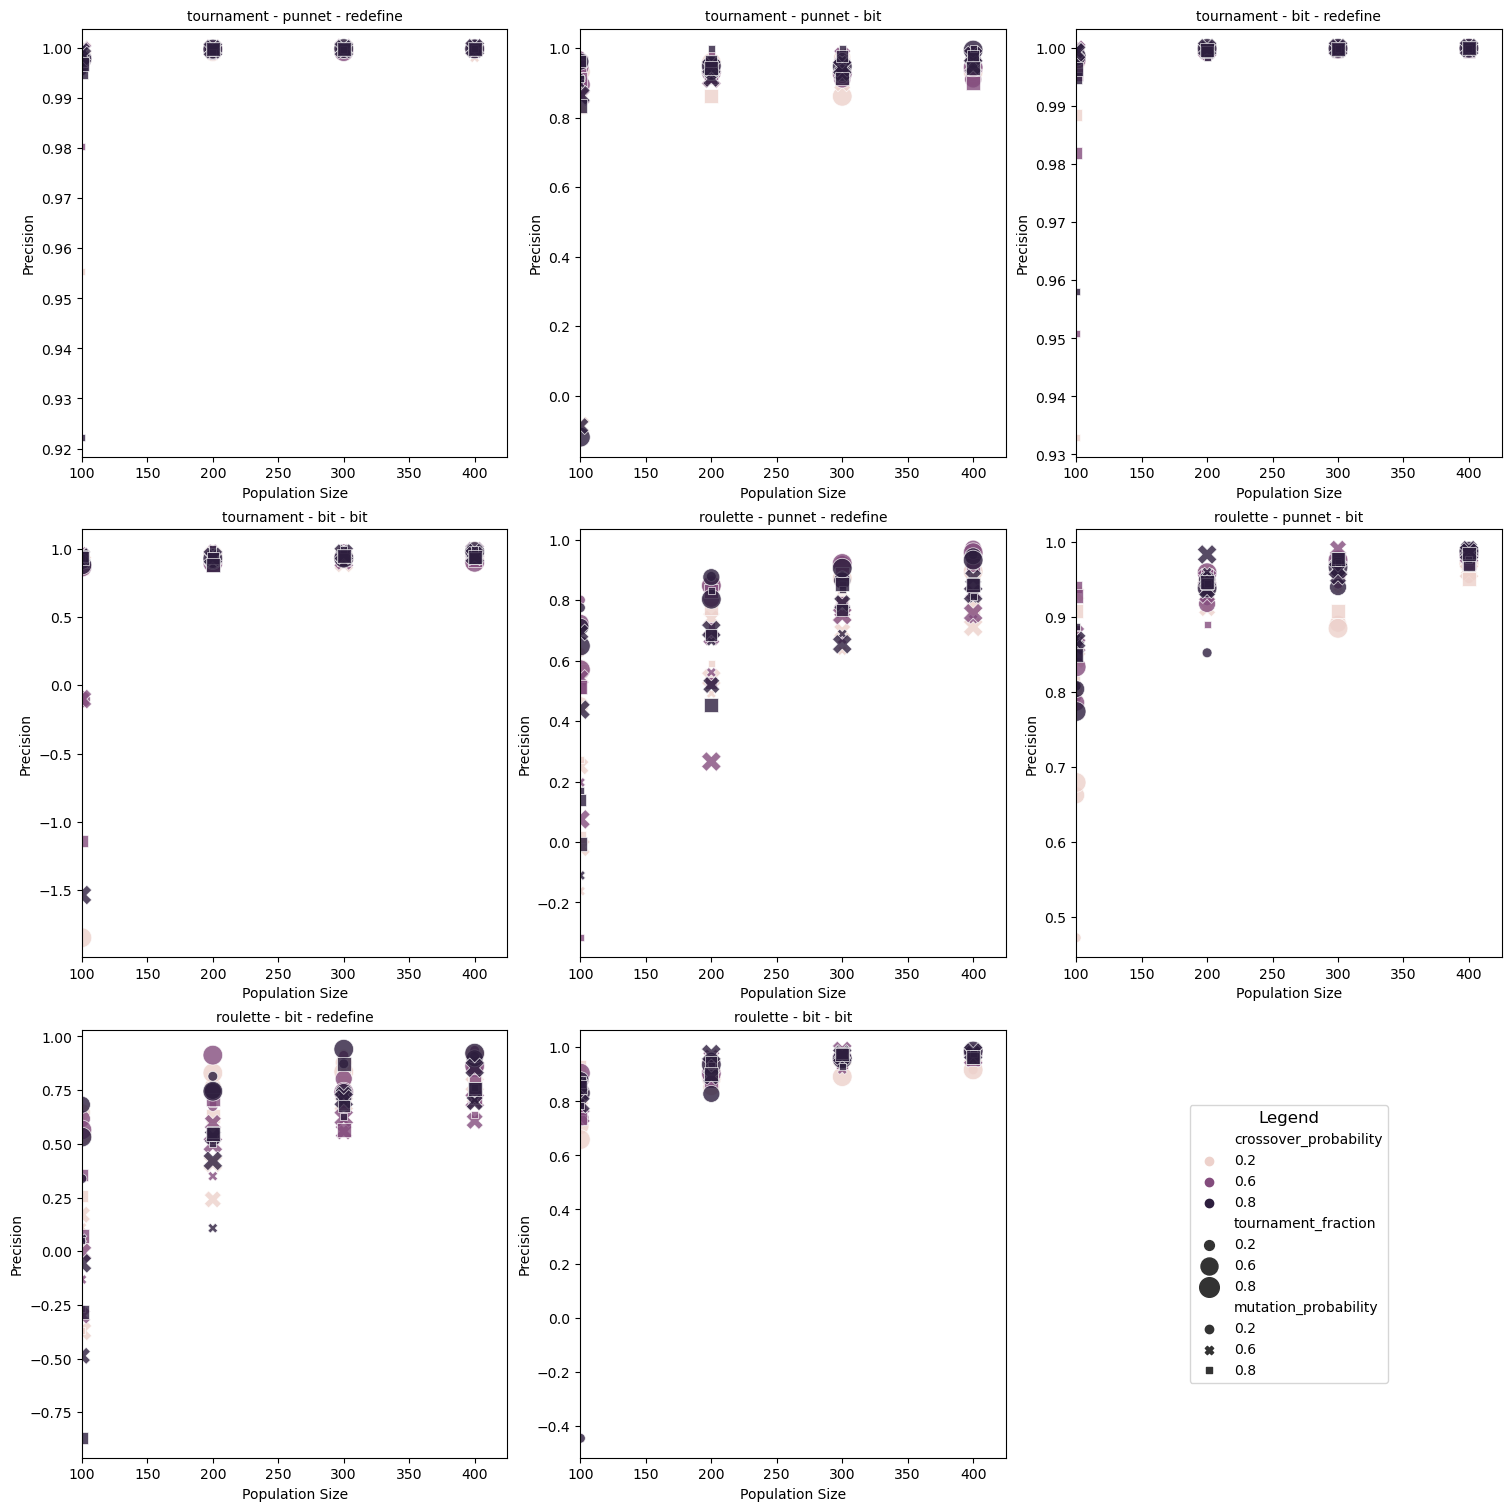
\includegraphics[width=\textwidth]{overall.png}
    \caption{Precision vs Population size for all combinations analyzed}
    \label{fig:overall}
\end{figure}

\subsection{Execution Time}

Another critical parameter for solver performance is the execution time. As expected, execution time increases with population size. Interesting is the formation of "clusters" that become more distinct as the population grows, as shown in Figure \ref{fig:TPR_ex} for the TPR method. Based on this observation, the analysis will proceed by focusing on the largest population sizes and the top $5\%$ combinations for execution time.

It is also worth noting that larger populations tend to produce higher accuracy, as illustrated in Figure \ref{fig:precision}.

\begin{figure}[H]
    \centering
    % First image
    \begin{subfigure}[b]{0.45\textwidth}
        \centering
        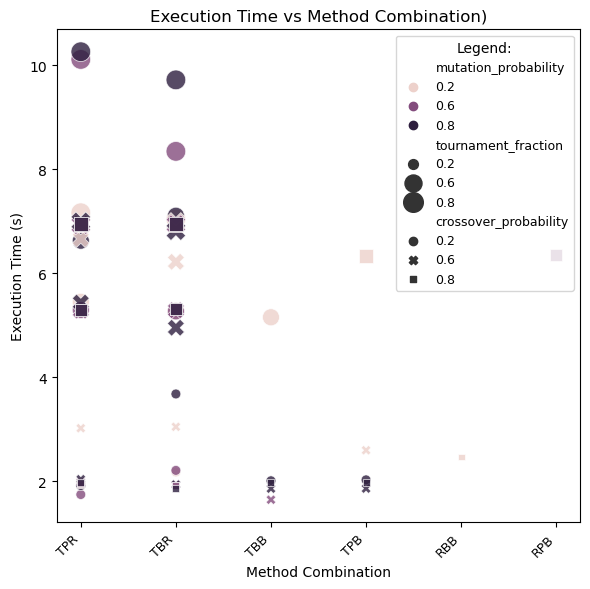
\includegraphics[width=\textwidth]{execution_time.png}
        \caption{Execution Times}
        \label{fig:Pop_sizes}
    \end{subfigure}
    \hfill
    % Second image
    \begin{subfigure}[b]{0.45\textwidth}
        \centering
        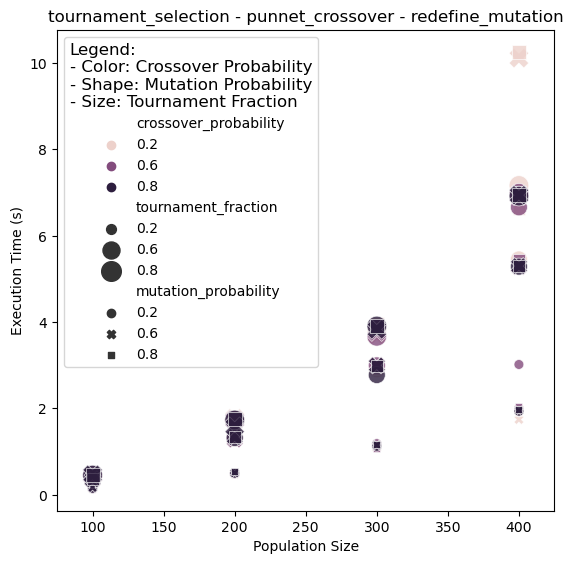
\includegraphics[width=\textwidth]{TPR_example.png}
        \caption{TPR Example}
        \label{fig:TPR_ex}
    \end{subfigure}
    \caption{Execution time for all combinations with $a>0.99$ based on methods \ref{fig:Pop_sizes} and execution time influenced by all parameters for the TPR method in particular \ref{fig:TPR_ex}.}
    \label{fig:comparison}
\end{figure}

\begin{figure}[H]
    \centering
    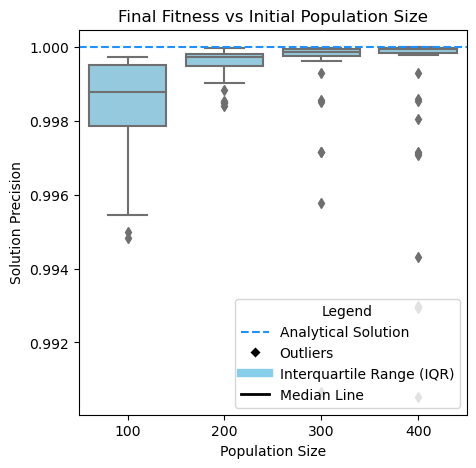
\includegraphics[width=0.5\textwidth]{precision_vs_pop.png}
    \caption{Precision vs Population size for all combinations analyzed}
    \label{fig:precision}
\end{figure}

\subsection{Parameter Effects}

The impact of input parameters on the results can now be examined in more detail. All the configurations with high precision and reasonably fast execution times share a tournament fraction of $20\%$.

As shown in Figure \ref{fig:mutation}, lower mutation probabilities reduce variation in the solution but can slightly compromise precision. This suggests that a finer analysis of this parameter towards low values might reveal an optimal balance.

For crossover, Figure \ref{fig:crossover} illustrates that higher probabilities improve solution quality. Compared to $p_C = 0.8$, lower probabilities exhibit smaller deviations but reduced precision. Increasing the probability to $0.6$ improves precision but introduces slightly larger deviations. Further exploration of higher values could provide deeper insights into the optimal setting for this parameter.

\begin{figure}[H]
    \centering
    % First image
    \begin{subfigure}[b]{0.35\textwidth}
        \centering
        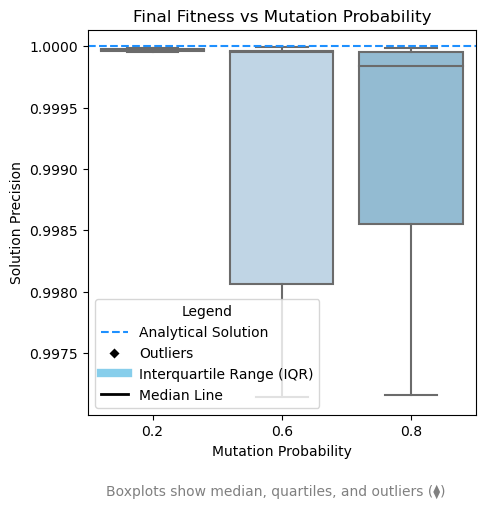
\includegraphics[width=\textwidth]{mutation.png}
        \caption{Precision vs Mutation Probability}
        \label{fig:mutation}
    \end{subfigure}
    \hfill
    % Second image
    \begin{subfigure}[b]{0.35\textwidth}
        \centering
        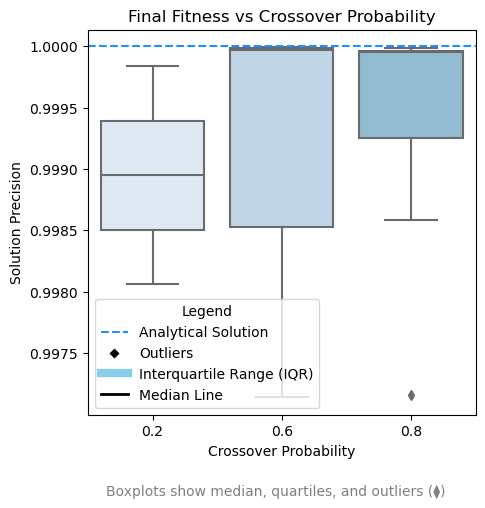
\includegraphics[width=\textwidth]{crossover.png}
        \caption{Precision vs Crossover Probability}
        \label{fig:crossover}
    \end{subfigure}
\end{figure}
Finally, we can now see a comparison between the best combinations so far.
\begin{figure}[H]
    \centering
    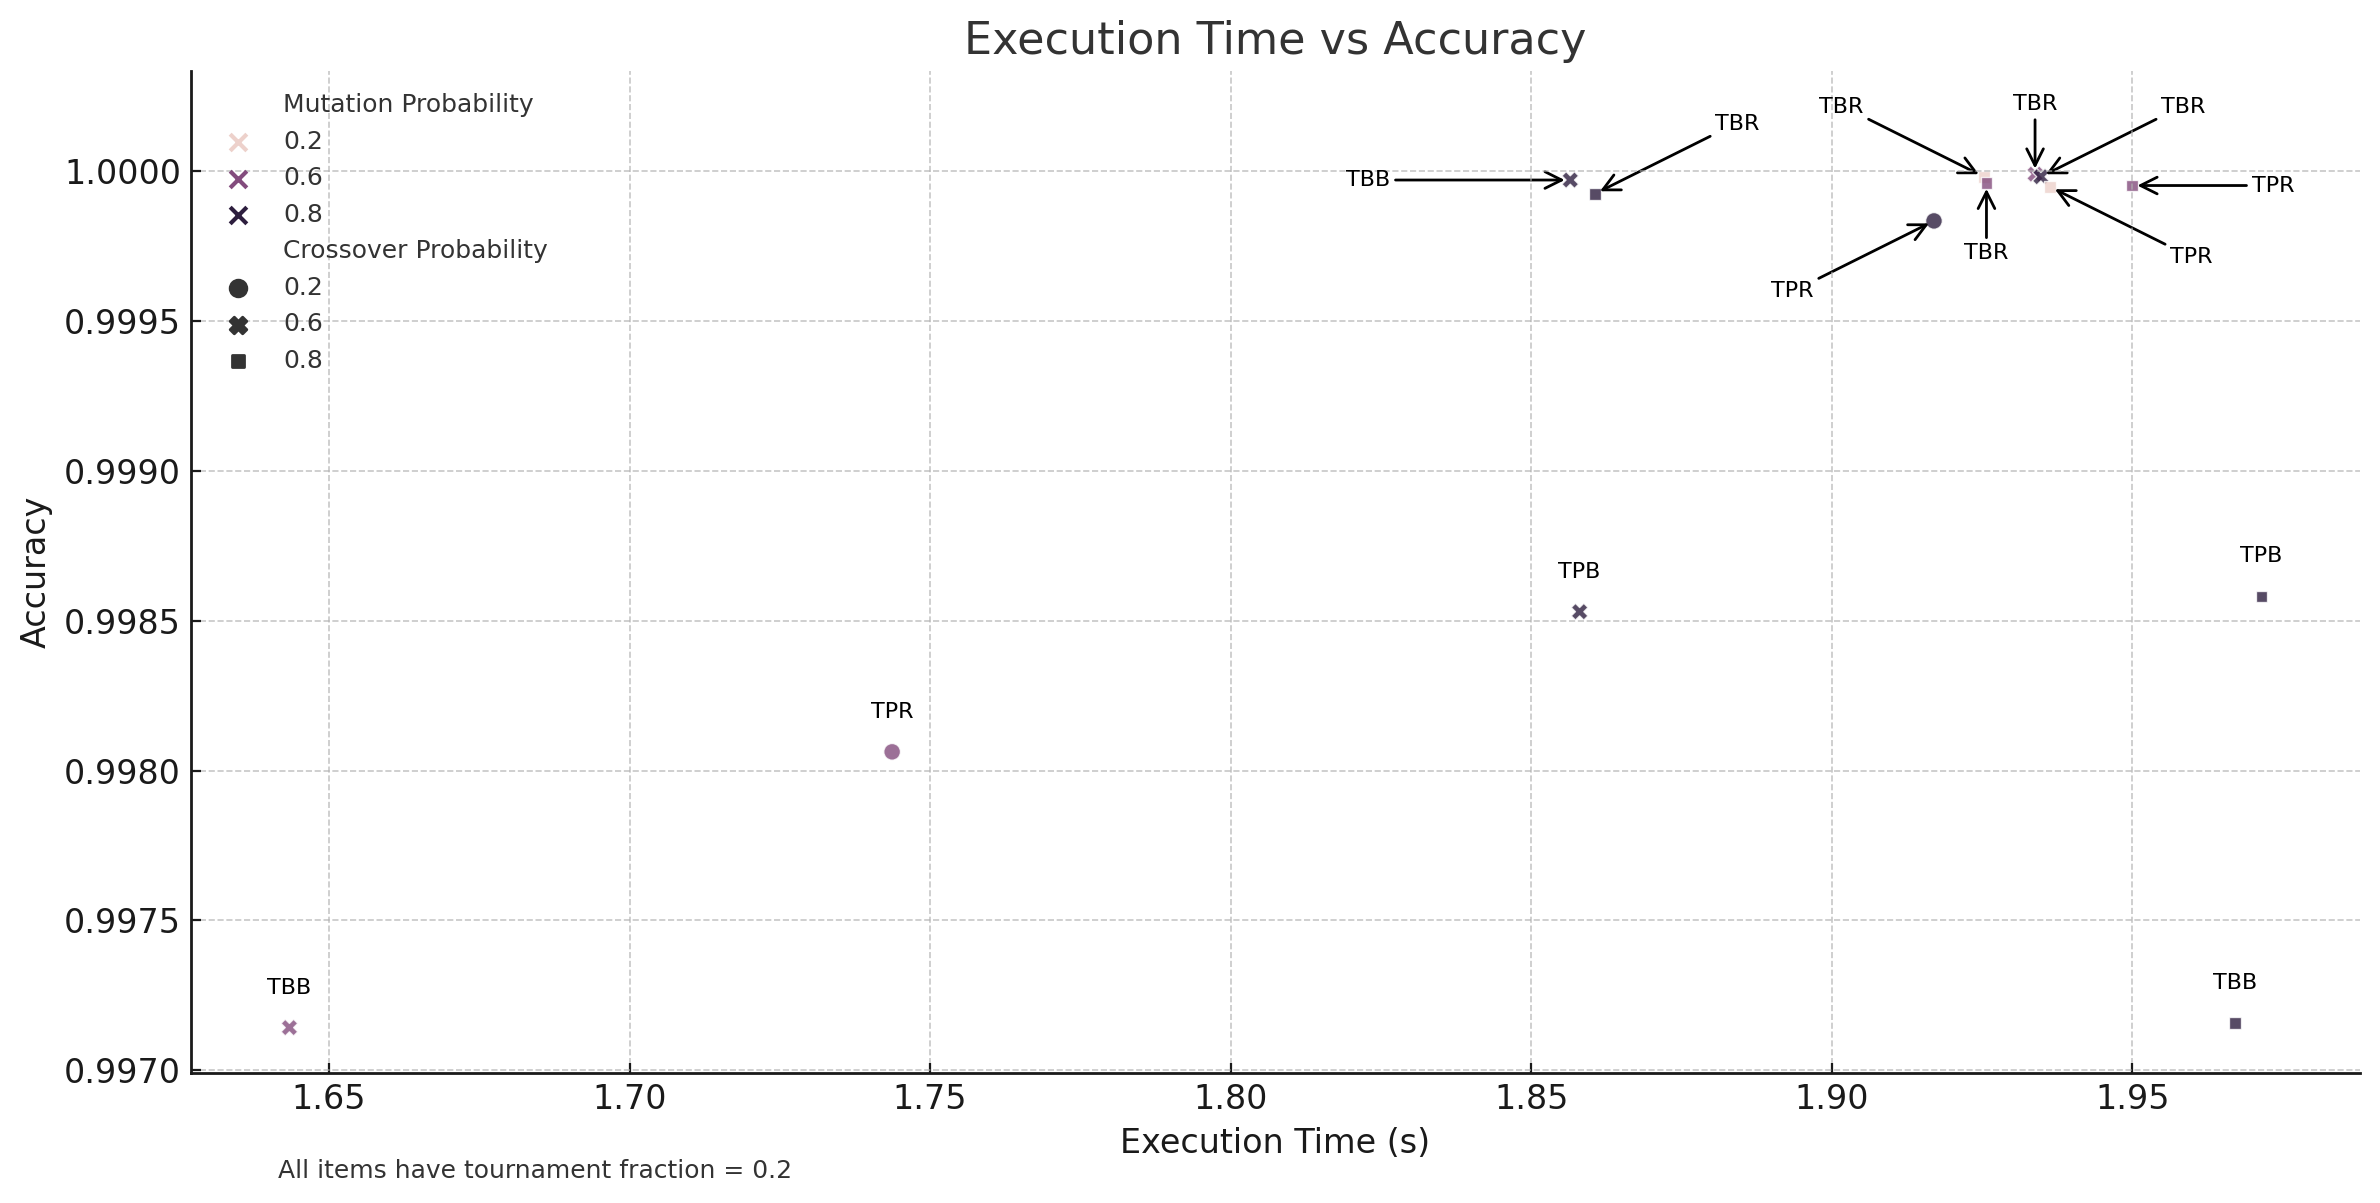
\includegraphics[width=\textwidth]{final.png}
    \caption{Execution time versus accuracy for optimal configurations.}
    \label{fig:final}
\end{figure}

\section{Results and Conclusion}

For the final run, the model providing the best balance between accuracy and execution time was chosen from the configurations tested. The selected parameters are as follows:

\begin{itemize} \item Population size: 400 individuals. \item Crossover probability: 0.6. \item Mutation probability: 0.6. \item Selection: Tournament selection. \item Crossover: Bit crossover. \item Mutation: Redefine mutation. \end{itemize}

The solver consistently converged to solutions near the global minimum of $-78.3323 \pm 0.0003$ with the following statistics: \begin{itemize} \item Average solution coordinates: $x = -2.9035 \pm 0.0011$, $y = -2.9036 \pm 0.0011$. \item Average execution time: $1.92 \pm 0.13$ seconds. \end{itemize} 

The algorithm achieved high accuracy and efficiency, converging reliably near the global minimum. The findings highlight the importance of careful parameter tuning to balance precision and execution time. Future work could further refine these results by exploring additional parameter values or applying the algorithm to more complex problems.

\end{document}
